\section{Ciberseguridad}

La ciberseguridad y la integridad estructural del código fuente representan pilares no negociables en la arquitectura de SocioUnido. Dado que la plataforma opera como un ecosistema integral de gestión para clubes de fútbol, procesando flujos financieros (cobro de cuotas, venta de entradas), información personal sensible del padrón de socios (PII) y gestionando controles de acceso físicos masivos, cualquier vulnerabilidad o fallo arquitectónico podría resultar en fugas de capital, interrupciones operativas severas o daños reputacionales irreparables para las instituciones.

Para garantizar la máxima fiabilidad a todos los niveles, el ciclo de vida del desarrollo de software de SocioUnido incorpora un enfoque proactivo de DevSecOps. Este paradigma trasciende la simple revisión manual, implementando herramientas de análisis estático, escaneo continuo de dependencias y monitoreo centralizado de calidad, asegurando que la seguridad sea un atributo inherente desde la fase de codificación hasta el despliegue en producción.

\subsection{Protección proactiva de dependencias: Implementación de Dependabot}

En el ecosistema moderno de desarrollo de software, especialmente en arquitecturas basadas en microservicios, los proyectos dependen de una vasta y compleja red de librerías y paquetes de terceros (el \textit{Supply Chain} de software). Estas dependencias, fundamentales para la agilidad del desarrollo, son frecuentemente el vector de ataque principal para la inyección de vulnerabilidades conocidas (CVEs - \textit{Common Vulnerabilities and Exposures}).

Para mitigar este riesgo de forma automatizada, la organización de GitHub de SocioUnido integra \textbf{Dependabot} en la totalidad de sus repositorios de desarrollo. La vitalidad de esta herramienta reside en su capacidad para actuar como un auditor de seguridad continuo e incansable:

\begin{itemize}
    \item \textbf{Monitoreo continuo:} Dependabot escanea ininterrumpidamente los manifiestos de dependencias (tales como \texttt{Gemfile.lock}, \texttt{package-lock.json}, o \texttt{requirements.txt} dependiendo del microservicio) cruzando las versiones utilizadas contra bases de datos globales de vulnerabilidades actualizadas en tiempo real.
    \item \textbf{Resolución automatizada:} Al detectar que un microservicio de SocioUnido (por ejemplo, el módulo de Pagos o el de Autenticación) está utilizando una versión de una librería con una brecha de seguridad pública, Dependabot no solo alerta al equipo, sino que genera automáticamente un \textit{Pull Request} (PR) proponiendo la actualización exacta a la versión mínima segura. Esto reduce el tiempo medio de remediación (MTTR) de días a horas.
    \item \textbf{Mantenimiento de la estabilidad:} Al combinarse con nuestra integración continua (CI), cada PR generado por Dependabot dispara automáticamente la batería de pruebas unitarias y de integración. Esto garantiza que la actualización de seguridad no rompa la lógica de negocio ni genere regresiones, permitiendo al equipo fusionar (\textit{merge}) el parche con total confianza.
\end{itemize}

\newpage

\subsection{Inspección y calidad centralizada: El rol estratégico de SonarCloud}

Mientras que Dependabot audita el código de terceros, la integridad, seguridad y mantenibilidad del código \textit{propio} desarrollado por el equipo requiere un análisis de caja blanca de extrema profundidad. Para este propósito, SocioUnido ha integrado \textbf{SonarCloud} como su motor principal de Análisis Estático de Código (SAST) y control de calidad.

La implementación de SonarCloud es vital para el proyecto por tres motivos fundamentales:

\begin{enumerate}
    \item \textbf{Detección Temprana de Vulnerabilidades Lógicas y \textit{Security Hotspots}:} Durante el flujo de Integración Continua (activado vía GitHub Actions en cada \textit{commit} o \textit{Pull Request}), SonarCloud analiza el código en busca de patrones peligrosos, fallos de inyección (SQLi, XSS), exposición accidental de credenciales o lógicas criptográficas débiles. Al identificar un riesgo, bloquea el despliegue mediante un \textit{Quality Gate} fallido, impidiendo que el código vulnerable llegue al entorno de producción.
    \item \textbf{Control de Deuda Técnica y \textit{Code Smells}:} Más allá de la seguridad pura, el sistema evalúa la mantenibilidad del software. Identifica código duplicado, lógicas excesivamente complejas (alta complejidad ciclomática) y desviaciones de los estándares de la industria (\textit{code smells}). Esto cuantifica la ``deuda técnica'' en horas de remediación, permitiendo al equipo de desarrollo priorizar la refactorización y mantener un código base limpio y escalable, fundamental para la posterior integración con los sistemas físicos de los estadios.
    \item \textbf{Trazabilidad a través del Repositorio \texttt{.github}:} La arquitectura descentralizada de SocioUnido (múltiples microservicios, frontends, APIs) presenta el desafío de la fragmentación de la información. Para resolver esto, hemos configurado un repositorio central especial denominado \texttt{.github}. Este repositorio actúa como la \textbf{torre de control y visualización centralizada} del proyecto. Mediante archivos \texttt{README} dinámicos y tableros integrados en \texttt{.github}, el equipo expone los \textit{badges} (insignias) y reportes consolidados de SonarCloud para \textit{todos} los repositorios involucrados. Esta vista panorámica es invaluable, ya que permite a cualquier miembro del equipo (o auditor externo) verificar de un vistazo el estado global de salud del ecosistema completo, así como profundizar en las métricas particulares (Bugs, Vulnerabilidades, Cobertura de Tests) de un microservicio específico sin necesidad de navegar por múltiples paneles aislados.
\end{enumerate}

En conclusión, la sinergia entre el escaneo de dependencias (Dependabot), la auditoría profunda de código fuente (SonarCloud) y la orquestación centralizada (repositorio \texttt{.github}) conforma una barrera de defensa profunda. Esta metodología exhaustiva garantiza que la plataforma SocioUnido no solo responda eficientemente a las necesidades funcionales de los clubes, sino que lo haga sobre cimientos arquitectónicos resilientes, auditables y ciberseguros.

\newpage

\subsubsection{Reportes generados por SonarCloud}

\subsubsection*{Métricas de actividad (Commits, Pull Requests e Issues)}

\begin{figure}[htbp]
    \centering
    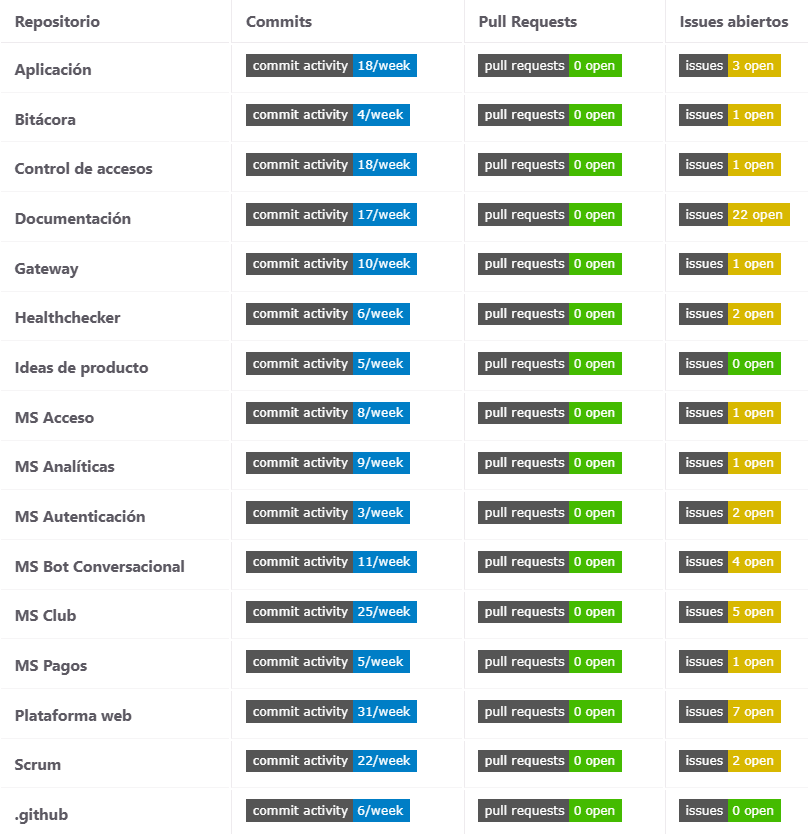
\includegraphics[width=\textwidth]{img/sonar/sonar-1.png}
    \caption{Métricas de actividad: Control de Commits, Pull Requests e Issues abiertos en el ecosistema de repositorios.}
    \label{fig:sonar-activity}
\end{figure}

\newpage

\subsubsection*{Reporte de estado (Quality Gate, bugs, seguridad, deuda técnica y duplicación de código)}

\begin{figure}[htbp]
    \centering
    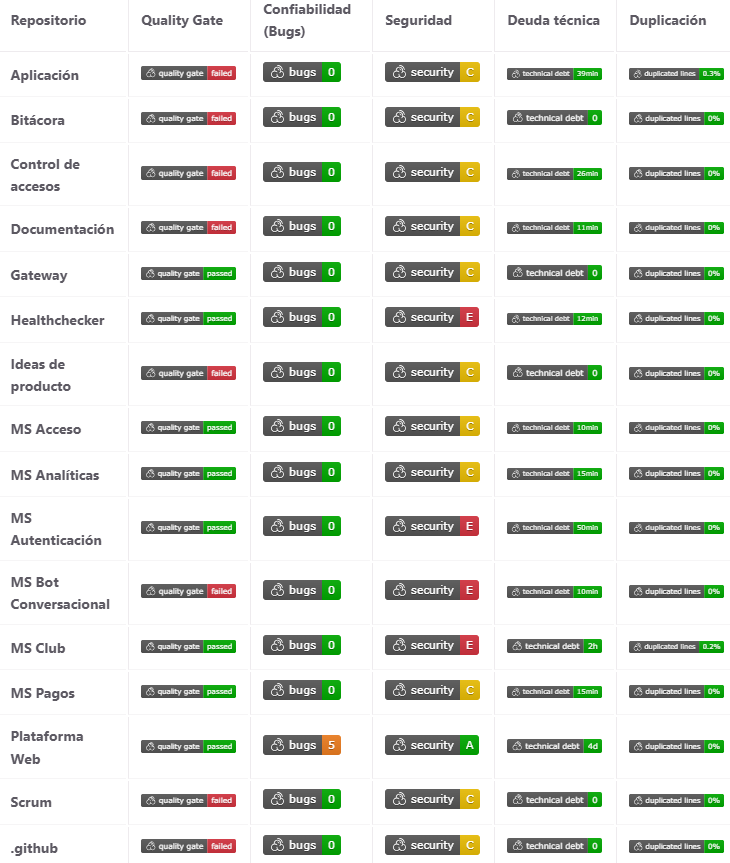
\includegraphics[width=0.95\textwidth]{img/sonar/sonar-2.png}
    \caption{Reporte de estado: Quality Gate, conteo de bugs, métricas de seguridad, deuda técnica y duplicación de código.}
    \label{fig:sonar-quality}
\end{figure}
